\documentclass{beamer}
\usepackage{tikz,amsmath,hyperref,graphicx,stackrel,animate,media9}
\usetikzlibrary{positioning,shadows,arrows,shapes,calc}
\newcommand{\argmax}{\operatornamewithlimits{argmax}}
\newcommand{\argmin}{\operatornamewithlimits{argmin}}
\mode<presentation>{\usetheme{Frankfurt}}
\AtBeginSection[]
{
  \begin{frame}<beamer>
    \frametitle{Outline}
    \tableofcontents[currentsection,currentsubsection]
  \end{frame}
}
\title{Lecture 6: Frequency Scales: Semitones, Mels, and ERBs}
\author{Mark Hasegawa-Johnson}
\date{ECE 417: Multimedia Signal Processing, Fall 2020}  
\begin{document}

% Title
\begin{frame}
  \maketitle
\end{frame}

% Title
\begin{frame}
  \tableofcontents
\end{frame}

%%%%%%%%%%%%%%%%%%%%%%%%%%%%%%%%%%%%%%%%%%%%
\section[Review]{Review: Equivalent Rectangular Bandwidth}
\setcounter{subsection}{1}

\begin{frame}
  \frametitle{Fletcher's Model of Masking, Reviewed}

  \begin{enumerate}
  \item The human ear pre-processes  the audio using a bank of bandpass filters.
  \item The power of the noise signal, in the  filter centered at $f_c$, is
    \[
    N_{f_c}=2\int_{0}^{F_S/2} R(f) |H_{f_c}(f)|^2 df
    \]
  \item The power of the tone is $T_{f_c}=A^2/2$, if the tone is at frequency $f_c$.
  \item If there is any band in which
    \[
    10\log_{10}\left(\frac{N_{f_c}+T_{f_c}}{N_{f_c}}\right)>1\mbox{dB}
    \]
    then the tone is audible.  Otherwise, not.
  \end{enumerate}
\end{frame}

\begin{frame}
  \frametitle{Equivalent rectangular bandwidth (ERB)}

  The frequency resolution of your ear is better at low frequencies.
  In fact, the dependence is roughly linear (Glasberg and Moore,
  1990):
  \[
  b \approx 0.108 f + 24.7
  \]
  These are often called (approximately) constant-Q filters, because
  the quality factor is
  \[
  Q = \frac{f}{b} \approx 9.26
  \]
  The dependence of $b$ on $f$ is not quite linear.  A more precise
  formula is given in (Moore and Glasberg, 1983) as:
  \[
  b = 6.23\left(\frac{f}{1000}\right)^2 + 93.39\left(\frac{f}{1000}\right)+28.52
  \]
\end{frame}

\begin{frame}
  \frametitle{Equivalent rectangular bandwidth (ERB)}

  \centerline{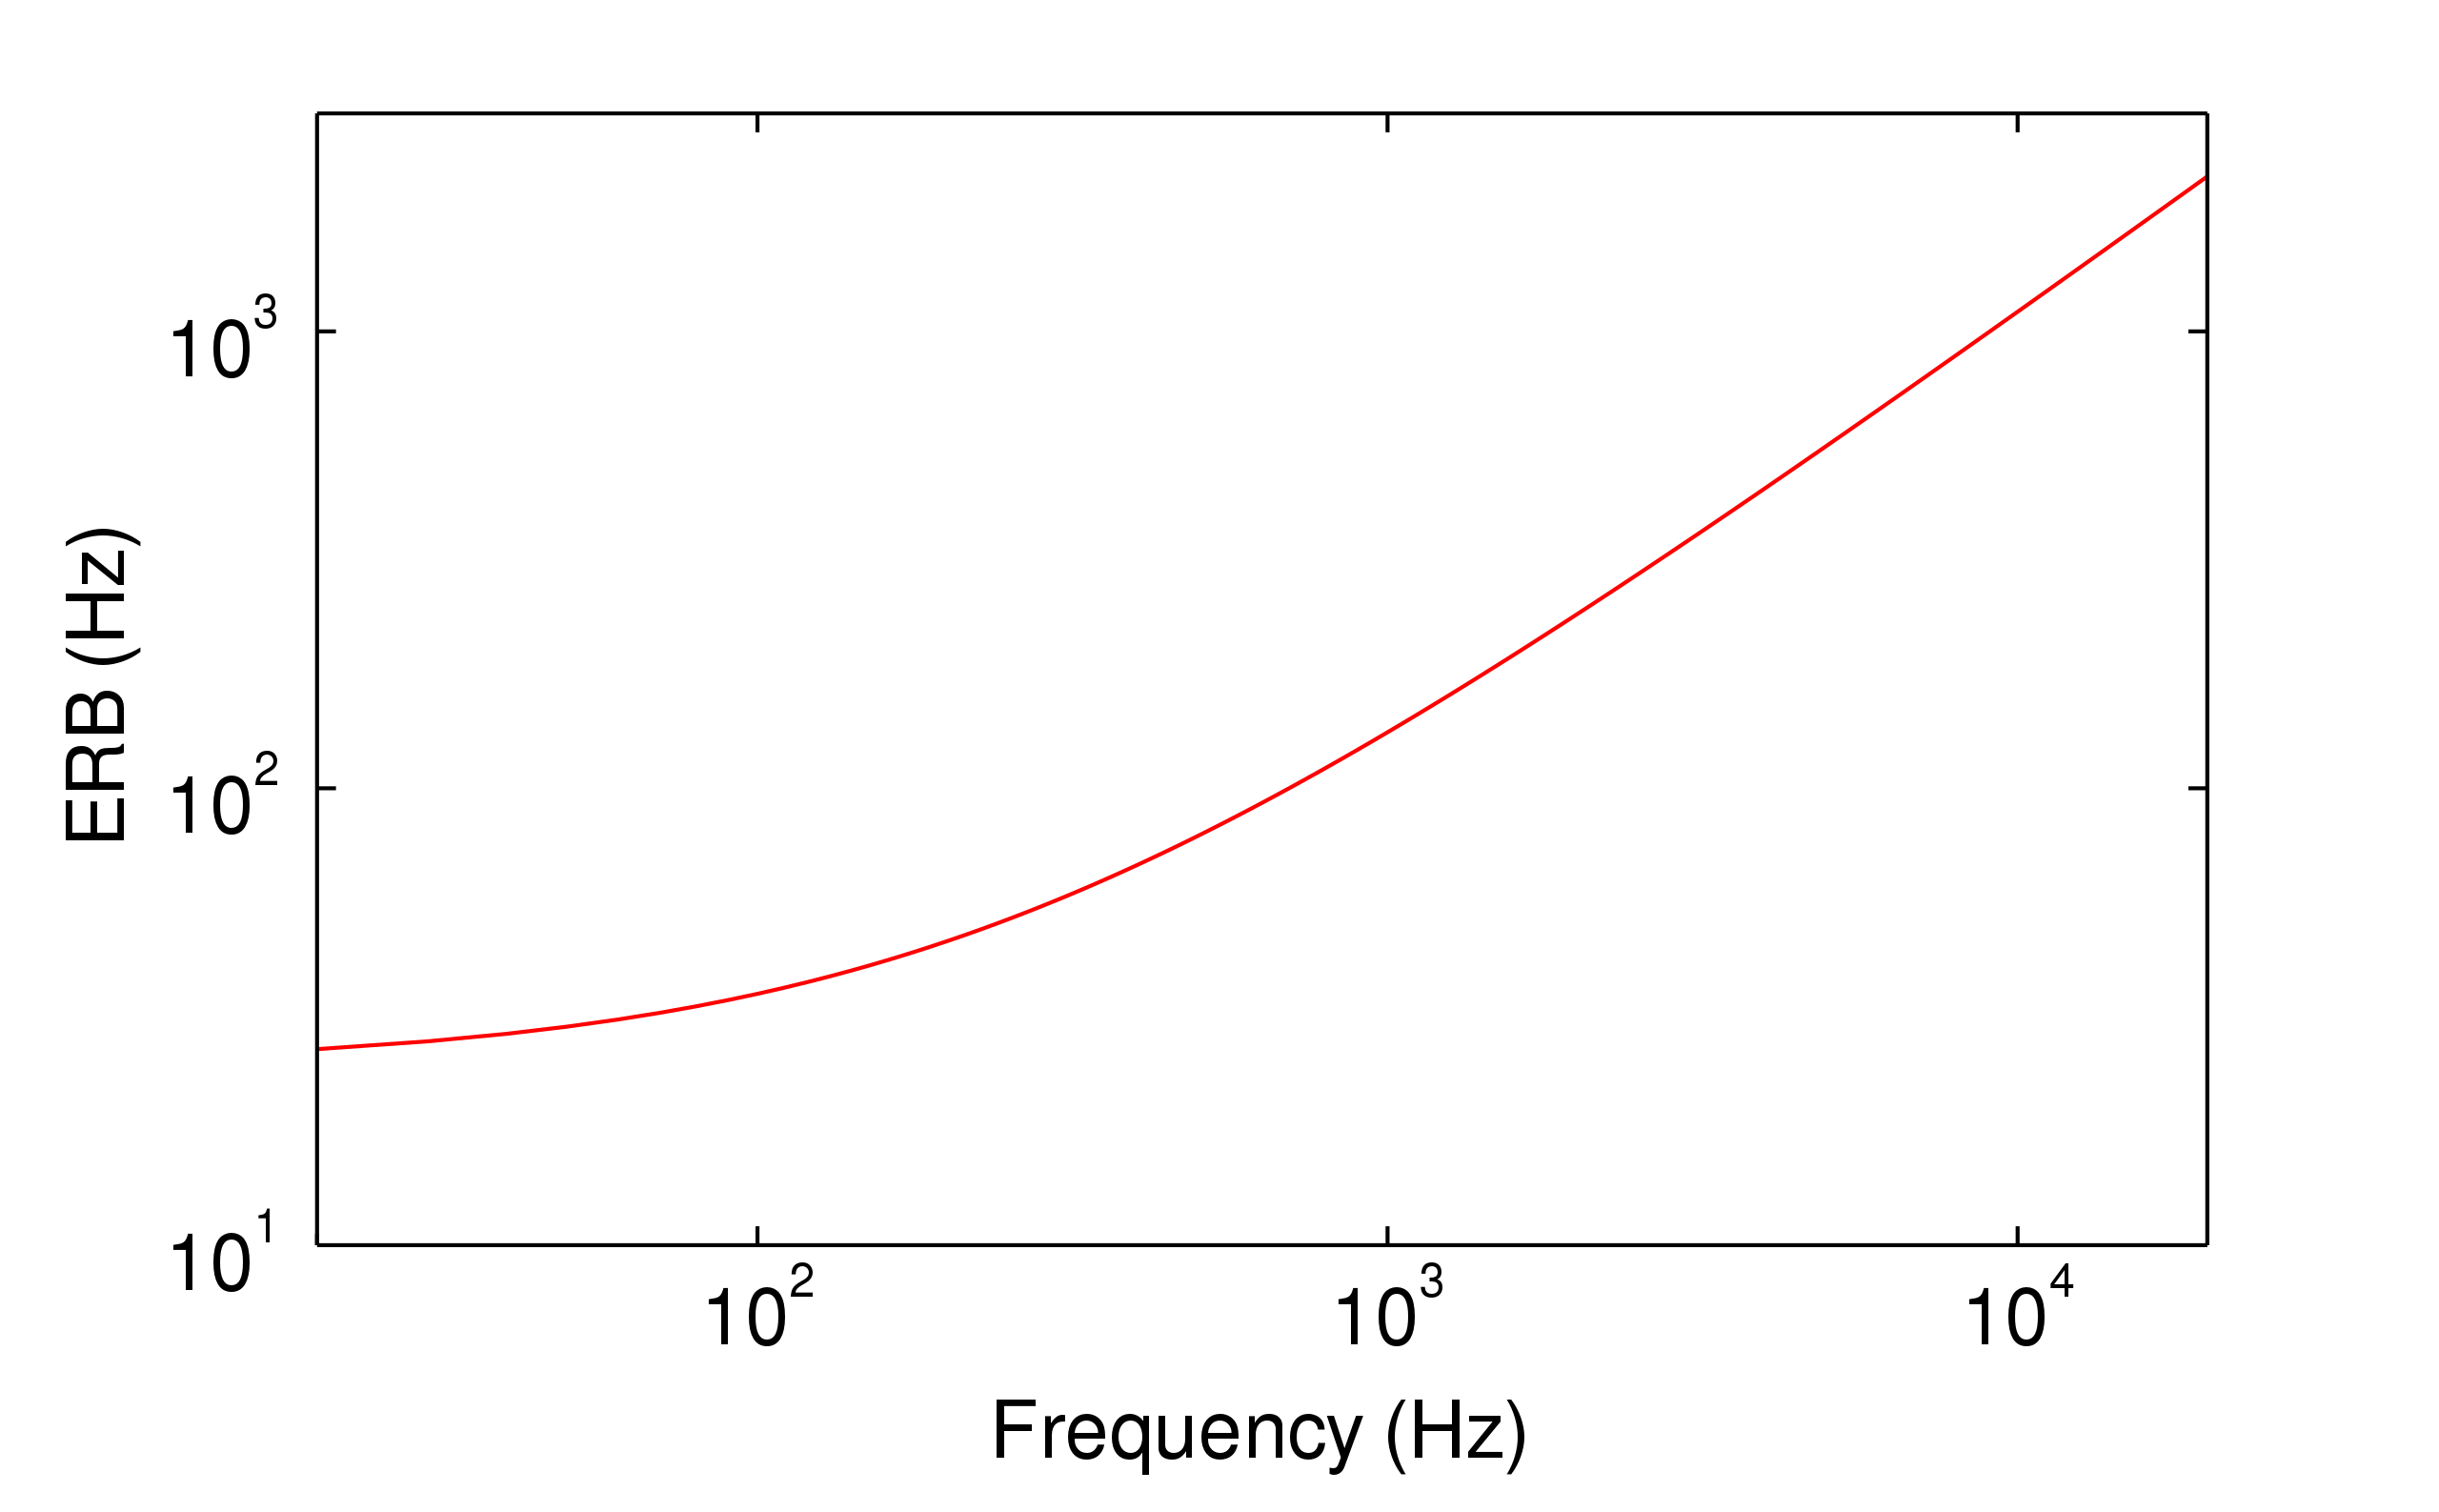
\includegraphics[height=2in]{../lec04/2560px-ERB_vs_frequency.png}}
  \begin{tiny}
    By Dick Lyon, public domain image 2009,
    \url{https://commons.wikimedia.org/wiki/File:ERB_vs_frequency.svg}
  \end{tiny}
\end{frame}

\begin{frame}
  \frametitle{The Gammatone Filter}

  The shape of the filter is not actually rectangular.  Patterson showed that it is
  \[
  |H(f)|^2 = \frac{1}{(b^2+(f-f_0)^2)^4}
  \]  
  He suggested modeling it as
  \[
  H(f) = \left(\frac{1}{b + j(f-f_0)}\right)^n + \left(\frac{1}{b + j(f+f_0)}\right)^n
  \]
  Whose inverse transform is a filter called a {\bf gammatone filter}.
  \[
  h(t) \propto t^{n-1} e^{-2\pi bt}\cos(2\pi f_0 t)u(t)
  \]
\end{frame}

\begin{frame}
  \frametitle{The Gammatone Filter: Spectrum}

  The top frame is a white noise, $x[n]$.  The middle frame is a
  gammatone filter at $f_c=1000$Hz, with a bandwidth of $b=128$Hz.
  The bottom frame is the filtered noise $y[n]$.

  \centerline{\includegraphics[height=2in]{../lec03/exp/gtfiltered_white_powerspectrum.png}}
\end{frame}
  
\begin{frame}
  \frametitle{The Gammatone Filter: Impulse Response}

  The top frame is a white noise, $x[n]$.  The middle frame is a
  gammatone filter at $f_c=1000$Hz, with a bandwidth of $b=128$Hz.
  The bottom frame is the filtered noise $y[n]$.

  \centerline{\includegraphics[height=2in]{../lec03/exp/gtfiltered_white_waveform.png}}
\end{frame}

\begin{frame}
  \frametitle{Frequency responses of the auditory filters}

  Here are the squared magnitude frequency responses ($|H(\omega)|^2$)
  of 26 of the 30000 auditory filters. I plotted these using the
  parametric model published by Patterson in 1974:
  \centerline{\includegraphics[height=2in]{../lec03/exp/gammatone_filterbank.png}}
\end{frame}

\begin{frame}
  \frametitle{Implications for Speech and Audio Recognition}

  \begin{itemize}
  \item Different human words must be audibly different.
  \item If a human being can't hear the difference, then they can't be different words.
  \item If humans can't hear small differences at high frequencies, then those differences
    can't possibly change the meaning of a word.
  \item For speech recognition, we should represent the low-frequency
    spectrum as precisely as the human ear represents it, and the
    high-frequency spectrum as imprecisely as the human ear represents
    it.
  \end{itemize}
\end{frame}

%%%%%%%%%%%%%%%%%%%%%%%%%%%%%%%%%%%%%%%%%%%%
\section[Semitones]{Musical Pitch: Semitones, and Constant-Q Filterbanks}
\setcounter{subsection}{1}

\begin{frame}
  \frametitle{Musical Pitch}
  \centerline{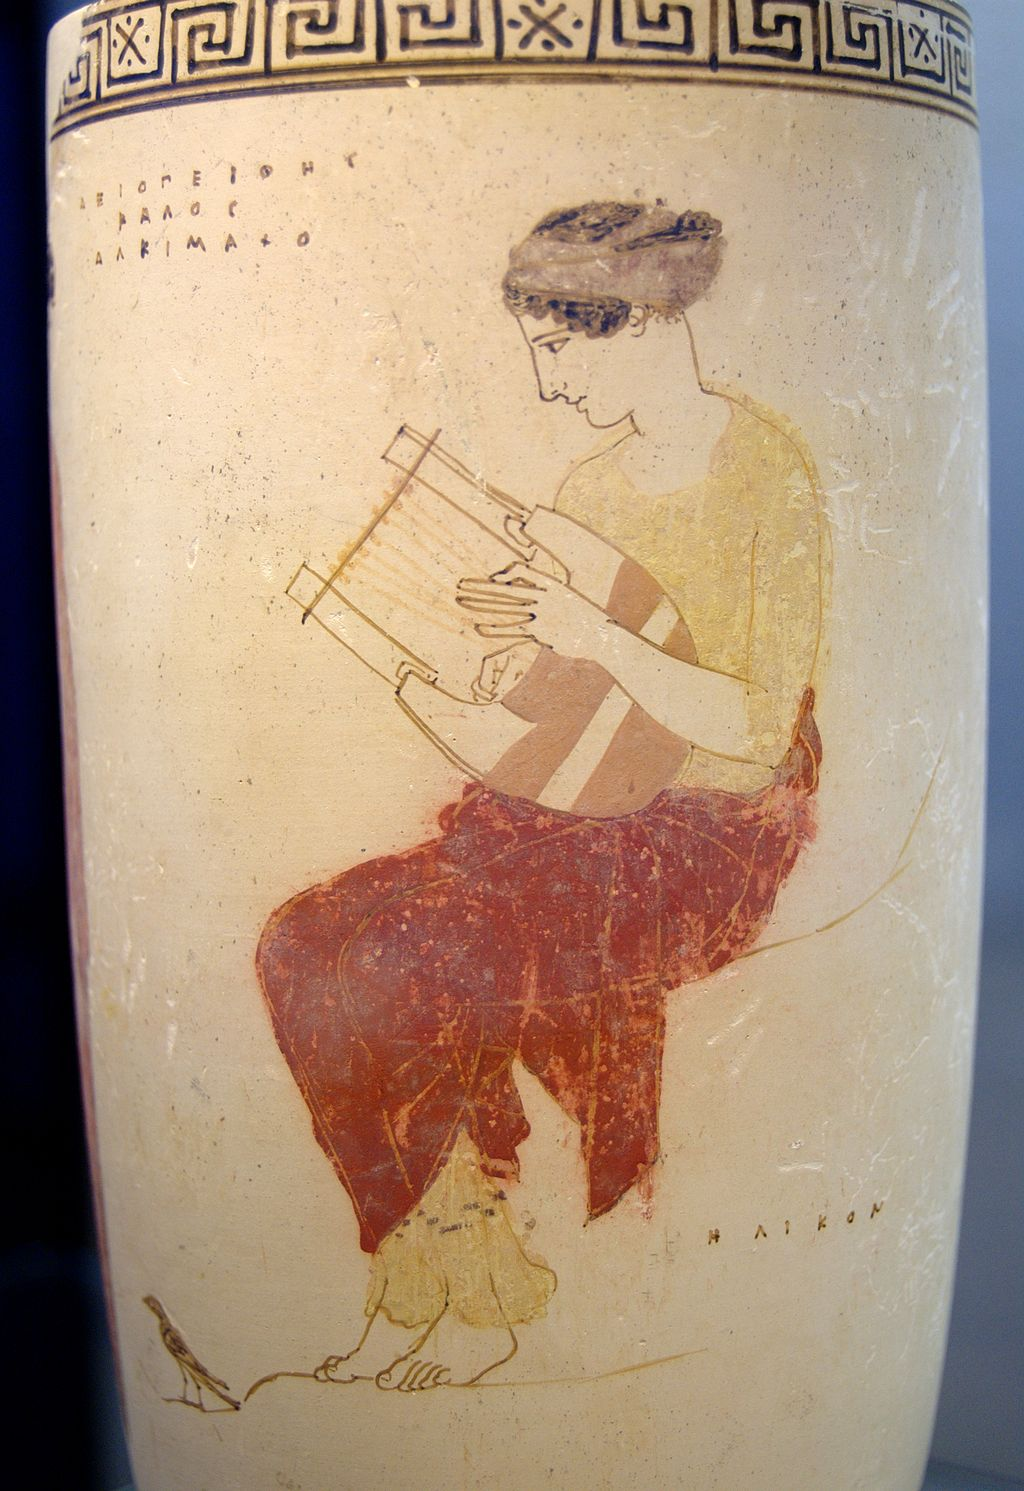
\includegraphics[height=2.5in]{helikon.jpg}}
  \begin{tiny}
    Muse playing the lyre, by the Achilles Painter.  Staatliche
    Antikensammlungen, public domain image by Bibi Saint-Pol,
    \url{https://commons.wikimedia.org/wiki/File:Mousai_Helikon_Staatliche_Antikensammlungen_Schoen80_n1.jpg}
  \end{tiny}
\end{frame}

\begin{frame}
  \frametitle{Pythagorean Tuning}
  \begin{itemize}
  \item Humans have always known that $f_2=2f_1$ (length of one string
    is twice the length of the other) means they are an octave apart
    (``same note'').
  \item A 3:2 ratio ($f_2=1.5f_1$) is a musical perfect fifth.
  \item Pythagoras is attributed with a system of tuning that created
    an 8-note scale by combining 3:2 and 2:1 ratios (``Pythagorean
    tuning''), used in some places until 1600.
  \end{itemize}
\end{frame}

\begin{frame}
  \frametitle{Equal-Tempered Tuning}

  Equal-tempered tuning divides the octave into twelve equal ratios.
  \begin{itemize}
  \item {\bf Semitones:} the number of semitones, $s$, separating two
    tones $f_2$ and $f_1$ is given by
    \[
    s = 12\log_2\left(\frac{f_2}{f_1}\right)
    \]
  \item {\bf Cents:} the number of cents, $n$, separating two tones
    $f_2$ and $f_1$ is given by
    \[
    n = 1200\log_2\left(\frac{f_2}{f_1}\right)
    \]
  \end{itemize}
\end{frame}

\begin{frame}
  \frametitle{Pythagorean vs. Equal-Tempered Tuning}
  \centerline{\fbox{\href{https://en.wikipedia.org/wiki/Pythagorean_tuning}{Pythagorean, Equal-Tempered, and Just Intonation}}}
\end{frame}

\begin{frame}
  \frametitle{Pythagorean vs. Equal-Tempered Tuning}
  \centerline{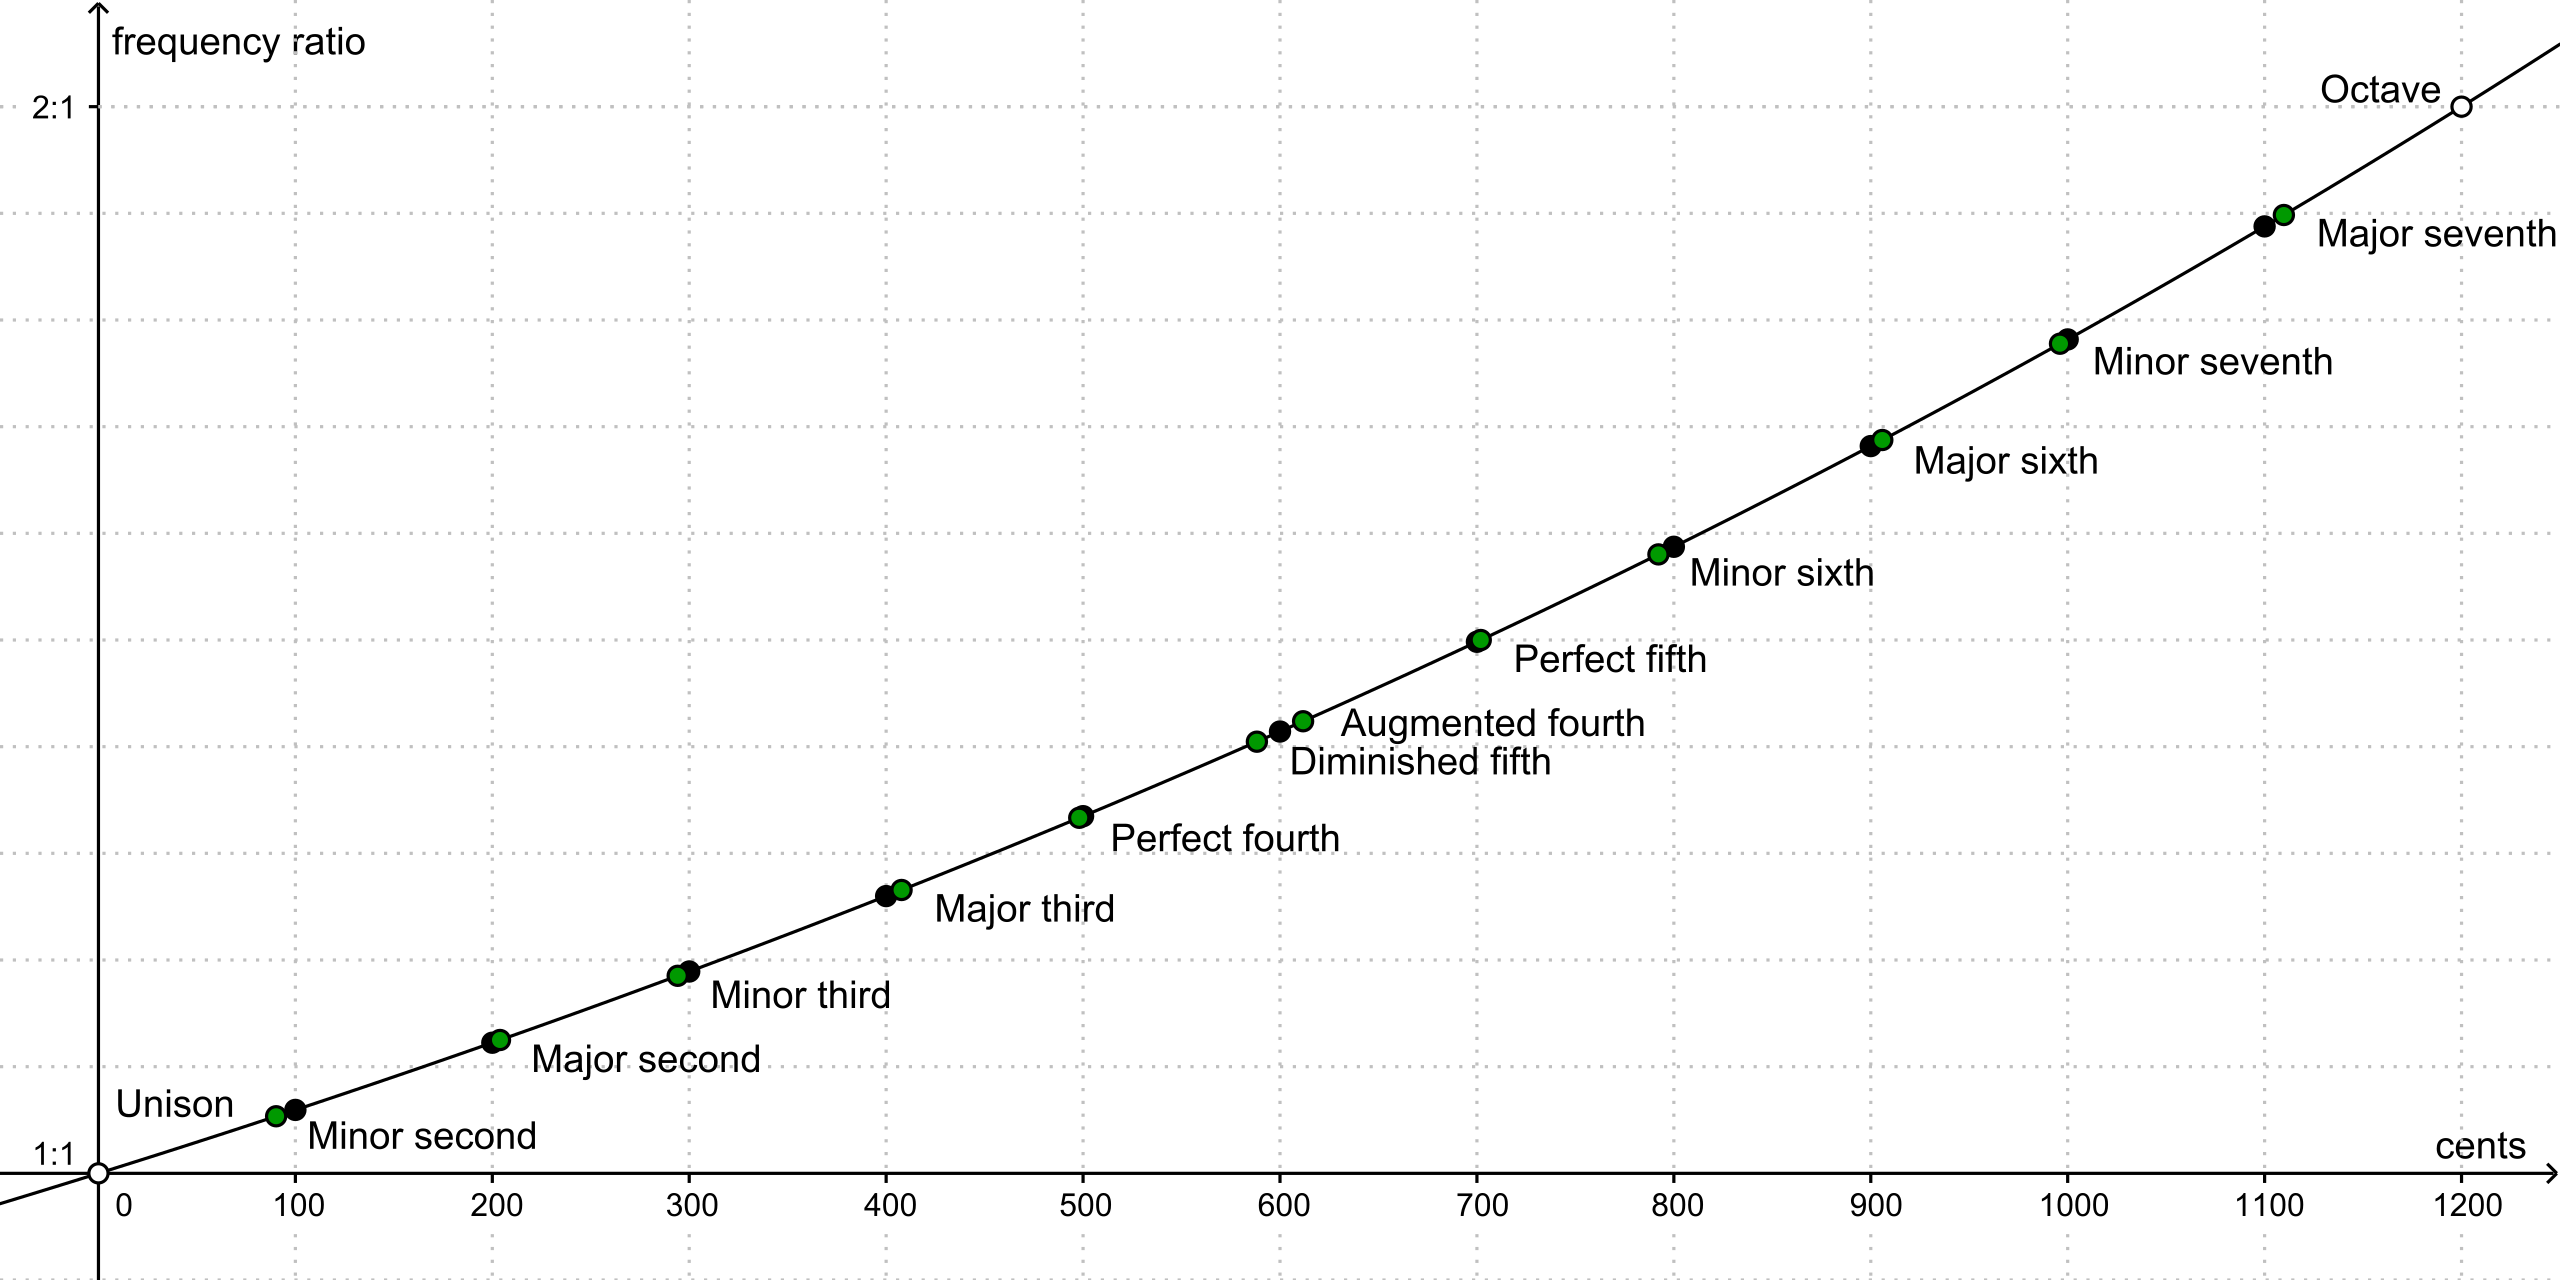
\includegraphics[height=2in]{Music_intervals.png}}
  \begin{tiny}
    By SharkD, public domain image,
    \url{https://commons.wikimedia.org/wiki/File:Music_intervals_frequency_ratio_equal_tempered_pythagorean_comparison.svg}
  \end{tiny}
\end{frame}

\begin{frame}
  \frametitle{Acoustic Features  on a Semitone Scale: the Constant-Q Transform}

  \begin{itemize}
  \item Gautham J. Mysore and Paris Smaragdis,
    \href{https://ieeexplore.ieee.org/document/4959583}{\underline{Relative pitch estimation of multiple instruments}}, ICASSP 2009
  \item Christian Sch\"{o}rkhuber, Anssi Klapuri and Alois Sontacchi,
    \href{https://www.cs.tut.fi/sgn/arg/klap/schoerkhuber-JAES-2013.pdf}{\underline{Audio Pitch Shifting Using the Constant-Q Transform}}, Journal of the Audio Engineering Society 61(7/8):562-572, 2013
  \item Massimiliano Todisco, H\'{e}ctor Delgado and Nicholas Evans,
    \href{https://pdfs.semanticscholar.org/1c8b/4e300f86555b514ec1e0c3fd58763524c2ac.pdf}{\underline{A New Feature for Automatic Speaker Verification} \underline{Anti-Spoofing: Constant Q Cepstral Coefficients}}, Speaker Odyssey 2016, pp. 283-290
  \end{itemize}
\end{frame}

\begin{frame}
  \frametitle{Constant-Q transform}

  Just like an STFT, suppose that we want our features to be
  \[
  X[k,n] = x[n]\ast h_k[n]
  \]
  but now suppose we want the filters to be spaced exactly one
  semitone apart, starting at note A1 on the piano:
  \[
  f_k = 55\times (2)^{k/12}
  \]
  and suppose that, instead of every filter having the same bandwidth,
  suppose we want the bandwidth, $b_k$, to be exactly one tone (one
  sixth of an octave).  That means we want the quality factor to be
  constant:
  \[
  Q = \frac{f_k}{b_k} = 6
  \]
\end{frame}
  
\begin{frame}
  \frametitle{Bandwidth of Rectangular \& Hamming windows}
  
  The rectangular window is
  \[
  w_R[n]=u[n]-u[n-N] \leftrightarrow
  W_R(\omega)=e^{-j\omega\frac{N-1}{2}}\frac{\sin(\omega N/2)}{\sin(\omega/2)}
  \]
  The Hamming window is
  \[
  w_H[n] = \left(0.54-0.46\cos\left(\frac{2\pi n}{N-1}\right)\right)w_R[n]
  \]
  We can estimate bandwidth by finding the frequency of the first null.  That would give
  \begin{align*}
    {\bf Rectangular}: &~~b =\frac{F_s}{N}\mbox{Hz} =\frac{2\pi}{N}\frac{\mbox{radians}}{\mbox{sample}}\\
    {\bf Hamming}: &~~b =\frac{2F_s}{N}\mbox{Hz} =\frac{4\pi}{N}\frac{\mbox{radians}}{\mbox{sample}}
  \end{align*}
\end{frame}

\begin{frame}
  \frametitle{Constant-Q transform}

  Putting it all together, we get the ``Constant Q Transform'' as:
  \[
  X_{CQT}[k,m] = x[n]\ast h_k[-n],~~~h_k[n]=w_k[n]e^{j\omega_k n}
  \]
  where $w_k[n]$ is a window with a length given by
  \[
  Q = \frac{f_k}{b_k},~~b_k=\frac{F_s}{N[k]}~~\Rightarrow N[k]=\frac{F_s}{f_k}Q
  \]
\end{frame}

      
%%%%%%%%%%%%%%%%%%%%%%%%%%%%%%%%%%%%%%%%%%%%
\section[Mel]{Perceived Pitch: Mels, and Mel-Filterbank Coefficients}
\setcounter{subsection}{1}

\begin{frame}
  \frametitle{Geometric pitch or perceived pitch?}

  \begin{itemize}
  \item Hertz: tones are equally spaced on a linear scale
  \item Semitones: tones are equally spaced on a logarithmic scale
  \item Mel: equally-spaced tones sound equally far apart, regardless of how high or
    low the pitch.
  \end{itemize}
\end{frame}
\begin{frame}
  \frametitle{A Scale for the Measurement of the Psychological Magnitude Pitch\\
    \begin{tiny}John E. Volkmann and Stanley S. Stevens\end{tiny}}

  Volkmann and Stevens used the following procedure:
  \begin{itemize}
  \item Play listeners a sequence of three notes, e.g.,
    \includemedia[addresource=threenotes.mp3,flashvars={source=threenotes.mp3&autoPlay=true}]{\fbox{Play}}{APlayer.swf}
  \item Ask the listener to choose a fourth note such that
    Note4-Note3 = Note2-Note1
  \item Define the mel-scale (short for ``melody'')  such that
    mel(Note4)-mel(Note3) = mel(Note2)-mel(Note1)
  \end{itemize}
\end{frame}

\begin{frame}
  \frametitle{The Mel Scale}

  Result: the Mel scale is roughly linear at low frequencies, roughly
  logarithmic at high frequencies.
  \[
  \mbox{Mel}(f) = 2595\log_{10}\left(1+\frac{f}{700}\right)
  \]
  \centerline{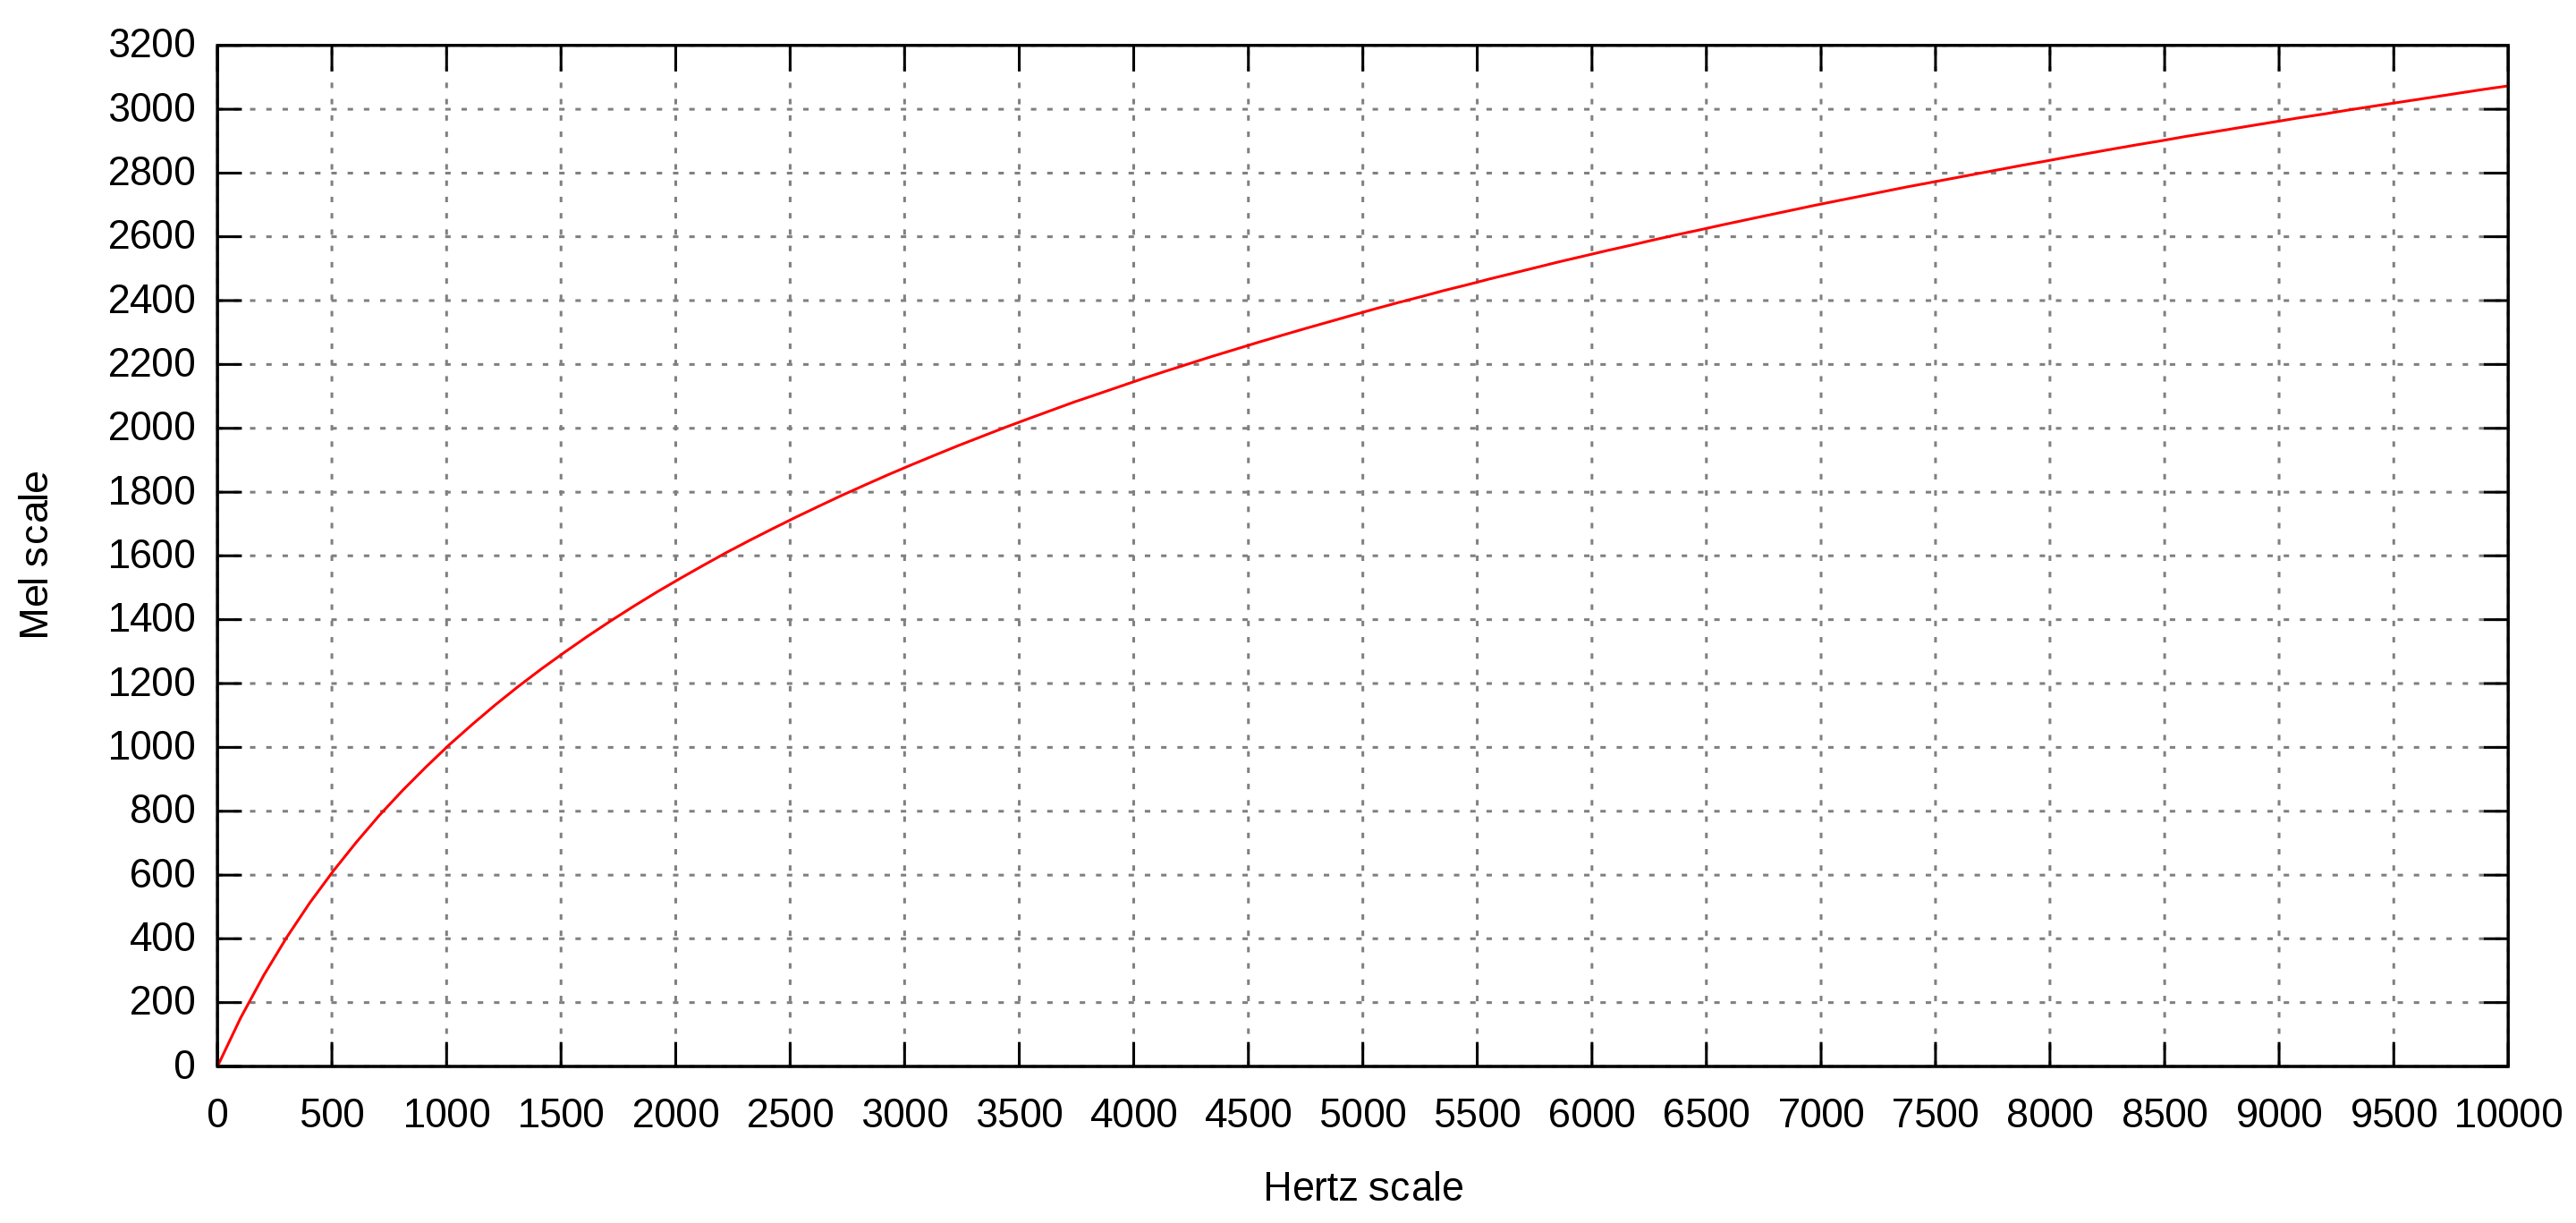
\includegraphics[height=1.25in]{Mel-Hz_plot.png}}
  \begin{tiny}
    By Krishna Vedala, GFDL,
    \url{https://commons.wikimedia.org/wiki/File:Mel-Hz_plot.svg}
  \end{tiny}
\end{frame}

\begin{frame}
  \frametitle{Acoustic Features on a Perceptual Scale: Mel-Frequency Cepstrum and Filterbank}
  \begin{itemize}
  \item {\bf MFCC}: Steven Davis and Paul Mermelstein,
    \href{https://ieeexplore.ieee.org/document/1163420}{\underline{Comparison of parametric representations} \underline{for monosyllabic word recognition in continuously spoken sentences}},
    IEEE Trans. ASSP 28(4):357-366, 1980
  \item {\bf Filterbank Coefficients:} Jinyu Li, Dong Yu, Jui-Ting Huang and Yifan Gong,
    \href{https://ieeexplore.ieee.org/abstract/document/6424210?casa_token=Ad3Ih5CvZIYAAAAA:5_LoLH71R6lGjlwiyUP54EI9dykCpk3hlPknh7ZdNGxMtKm_c1u13qIRGVa0WUnZlRj0f-9F}{Improving wideband speech recognition using mixed-bandwidth training data in CD-DNN-HMM}, 2012 IEEE SLT
  \item Beth Logan,
    \href{http://citeseerx.ist.psu.edu/viewdoc/download?doi=10.1.1.11.9216&rep=rep1&type=pdf}{\underline{Mel-Frequency Cepstral Coefficients for Music Modeling}}, ISMIR 2000
  \end{itemize}
\end{frame}

\begin{frame}
  \frametitle{Mel Frequency Filterbank Coefficients}

  Suppose $X[k,m]$ is the STFT.  The mel filterbank coefficients are
  $C[\ell,m] = \ln\left(\sum_k w_\ell[k] |X[k,m]|\right)$, where the
  weights, $w_\ell[k]$, are triangles:
  \centerline{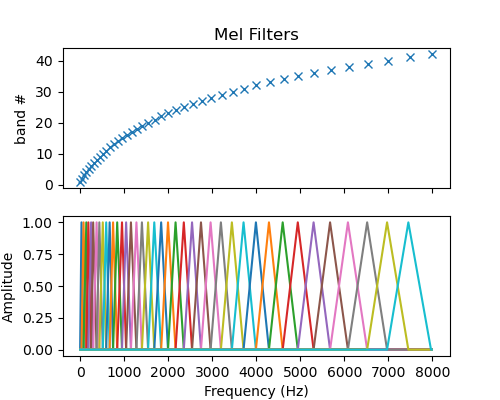
\includegraphics[height=2.5in]{mel_triangles.png}}
\end{frame}

\begin{frame}
  \frametitle{Mel vs.~Linear Frequency}

  Mel-frequency (on the right) stretches out the low frequencies more:
  
  \centerline{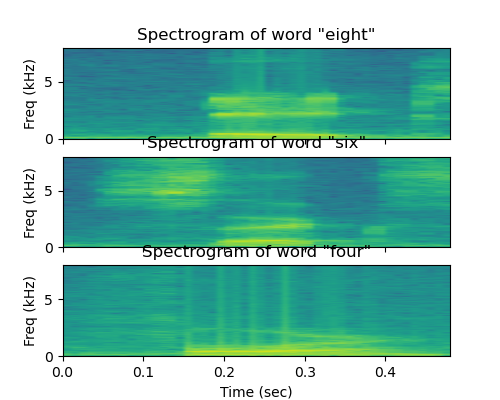
\includegraphics[height=2in]{spectrograms.png}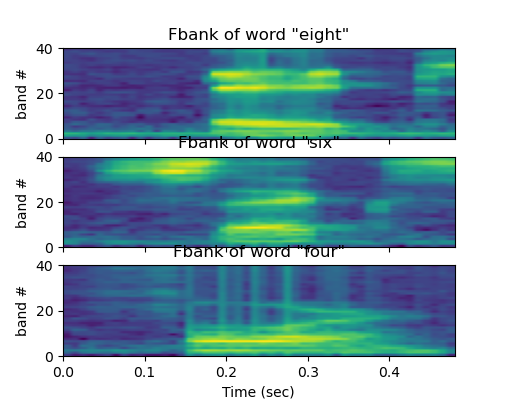
\includegraphics[height=2in]{fbank_spectrograms.png}}
\end{frame}

%%%%%%%%%%%%%%%%%%%%%%%%%%%%%%%%%%%%%%%%%%%%
\section[ERB]{Masking: Equivalent Rectangular Bandwidth Scale}
\setcounter{subsection}{1}

\begin{frame}
  \frametitle{Four frequency scales}

  \begin{itemize}
  \item Hertz: tones are equally spaced on a linear scale
  \item Semitones: tones are equally spaced on a logarithmic scale
  \item Mel: equally-spaced tones sound equally far apart, regardless of how high or
    low the pitch.
  \item ERBs: tones are $<1$ERB apart iff their auditory filters
    overlap, $\ge 1$ERB apart otherwise.
  \end{itemize}
\end{frame}

\begin{frame}
  \frametitle{ERB scale}

  Let $b$ be the equivalent rectangular bandwidth of a filter centered at $f$.
  We want to design a transform $e(f)$ so that
  \[
  e(f+b)\approx e(f)+1
  \]
  \[
  e(f+b)-e(f)  \approx 1
  \]
  \[
  \frac{e(f+b)-e(f)}{b} \approx \frac{1}{b}
  \]
  \[
  \frac{de}{df} = \frac{1}{b}
  \]
\end{frame}
\begin{frame}
  \frametitle{ERB scale}

  Using the linear approximation,
  \[
  \frac{de}{df} = \frac{1}{0.108 f + 24.7}
  \]
  we get
  \[
  e(f)  = \frac{1}{0.108}\ln\left(0.108f+24.7\right)
  \]
  \begin{itemize}
  \item It looks a lot like the mel scale!  Linear at low frequencies,
    logarithmic at high frequencies.
  \item ERBs cut over from linear scale to log-scale at $f=\frac{24.7}{0.108}=228$Hz,
    vs. Mels, which cut over at $f=700$Hz.
  \item The scale is $\frac{1}{0.108}=9.2$ERBs/octave: smaller than a tone, larger than
    a semitone.
  \end{itemize}
\end{frame}
\begin{frame}
  \frametitle{ERB scale}

  Using the quadratic approximation,
  \[
  \frac{de}{df} = \frac{1}{6.23\left(\frac{f}{1000}\right)^2 + 93.39\left(\frac{f}{1000}\right)+28.52}
  \]
  we get
  \[
  e(f)  = 11.17268 \ln\left(1+\frac{46.06538f}{f+14678.49}\right)
  \]
  \begin{itemize}
  \item Still linear at low frequencies,
    logarithmic at high frequencies.
  \item Linear-to-log cutover is $\frac{14678}{46}=319$Hz.
  \item 11.1 ERBs/octave: very close to a semitone
  \end{itemize}
\end{frame}

\begin{frame}
  \frametitle{ERBs vs.~Mel}

  \centerline{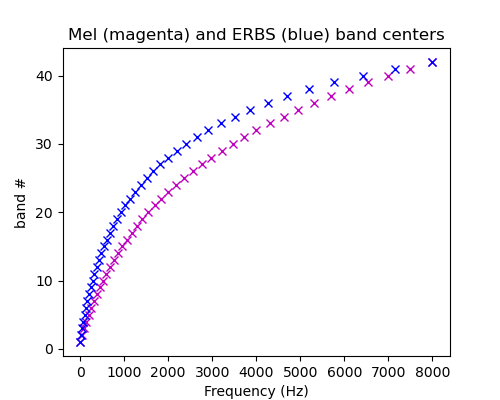
\includegraphics[height=3in]{mel_vs_erbs.png}}
\end{frame}

\begin{frame}
  \frametitle{Gammatone filterbank coefficients}

  Gammatone filterbank coefficients are computed as
  \[
  X[k,m] = x[n]\ast h_k[n]
  \]
  where we usually use Patterson's gammatone filterbanks:
  \[
  h_k(t) = t^3 e^{-2\pi b_kt}\cos(2\pi f_k t)u[n]
  \]
  Spaced equally on an ERBS scale:
  \[
  f_k = \mbox{ERB}^{-1}(k)
  \]
\end{frame}

\begin{frame}
  \frametitle{Gammatone filterbank coefficients for speech and audio}
  \begin{itemize}
  \item Many papers have had slightly better results using gammatone filterbank coefficients
    instead of mel filterbank coefficients, at the cost of greater computational cost
    (because gammatone coefficients are ${\mathcal O}\left\{N^2\right\}$, while
    MFFB are ${\mathcal O}\left\{N\log_2(N)\right\}$.
  \item Many recent papers since 2019 use learned filterbank
    coefficients, instead of gammatone filterbank coefficients.
  \end{itemize}
\end{frame}
  
%%%%%%%%%%%%%%%%%%%%%%%%%%%%%%%%%%%%%%%%%%%%
\section[Summary]{Summary}
\setcounter{subsection}{1}

\begin{frame}
  \frametitle{Summary}
  \begin{itemize}
  \item Semitones and Constant-Q filterbank:
    \begin{align*}
      f_k &= 55(2)^{k/12}\\
      X[k,n] &= x[n]\ast w_k[n]e^{j\omega_k n}
    \end{align*}
  \item Mel-Frequency Filterbank coefficients:
    \begin{align*}
      \mbox{Mel}(f) &= 2595\log_{10}\left(1+\frac{f}{700}\right)\\
      C[\ell,m] &= \ln\left(\sum_k w_\ell[k] |X[k,m]|\right)
    \end{align*}
  \item ERBS and Gammatone filterbank:
    \begin{align*}
      e(f)  &= 11.17268 \ln\left(\frac{1+46.06538f}{f+14678.49}\right)\\
      X[k,n] &= x[n]\ast \left(t^3 e^{-2\pi b_kt}\cos(2\pi f_k t)u[n]\right)
    \end{align*}
  \end{itemize}
\end{frame}
    
\end{document}

